%% LyX 2.3.0 created this file.  For more info, see http://www.lyx.org/.
%% Do not edit unless you really know what you are doing.
\documentclass[american]{article}
\usepackage[T1]{fontenc}
\usepackage[latin9]{inputenc}
\usepackage{textcomp}
\usepackage{amsmath}
\usepackage{amssymb}
\usepackage{graphicx}

\makeatletter
%%%%%%%%%%%%%%%%%%%%%%%%%%%%%% User specified LaTeX commands.
\usepackage{acl,url}
%\usepackage[a4paper,left=2.5cm,right=2cm,top=2.5cm,bottom=2.5cm]{geometry}
\usepackage{times}
\usepackage{latexsym}

\makeatother

\usepackage{babel}
\begin{document}
\global\long\def\argmax{\operatornamewithlimits{argmax}}

\global\long\def\argmin{\operatornamewithlimits{argmin}}


\title{Batch Active Learning for Text Classification and Sentiment Analysis}
\maketitle
\begin{abstract}
The performance of text classification with supervised models is tied
to quality and diversity of the data. The process of data collection
and labeling may involve a lot of resources. The intuitive and the
most standard approach is to sequentially extend a dataset with labeled
data until reaching satisfactory metrics. Active learning techniques
optimize the process of sequential unlabeled data selection, so that
the annotations would provide the most information about the dataset.
The problem of active learning becomes more complex when the sampling
is done in batches. In this paper we show a study of advanced batch
sampling techniques on text data and the problem of text classification
and sentiment analysis. The study compares i) baseline algorithm based
on agglomerative instance clustering with the subsequent sampling
from clusters given minimum margin of class probabilities ii) wam
start modifications of baseline techniques, and iii) Bayesian active
learning baseline modification thanks to their ability of better representation
of the classification uncertainty. The latter method in warm-start
version too. 

Transformers encoders show the state-of-the-art results in majority
of NLP tasks. In this article, we use RoBERTa for text encoding. The
methods are tested on three types datasets, context integrity (Kaggle
Gibberish dataset), fake news detection (Kaggle Fake News Detection
dataset) and sentiment classification (Twitter Sentiment140 and Amazon
Review Classification datasets). We show that both warm-start and
Bayesian baseline algorithm modifications outperform the state-of-art
approach. 
\end{abstract}

\section{Introduction}

The development of a text classifier on a new problem requires the
availability of the training data and their labels. Labeling involves
human annotators and a common practice is to label as many text documents
as possible, train a classifier and search for new data and labels
if the performance is unsatisfactory. Random choice of the documents
for the data set extension can be costly because the new documents
may not bring new information for the classification. Active learning
strategy aims to select among available unlabeled documents those
that the classifier is most uncertain about and queries an annotator
for their labels. Therefore, it has the potential to greatly reduce
the effort needed for the development of a new system. While it was
introduced almost two decades ago, recent improvements in deep learning
motivate our attempt to revisit the topic. For example, SVM-based
active learning approaches for text classification date back to 2001
{[}22{]} , where the superiority of active learning over random sampling
was demonstrated. Since deep recurrent and convolutional neural networks
achieve better classification results, Bayesian active learning methods
for deep networks gained popularity especially in image classification
{[}10{]}, {[}15{]} . The Bayesian approach is concerned with querying
labels for data for which the classifier predicts the greatest uncertainty.
 The uncertainty is quantified using the so-called acquisition function,
such as predictive entropy {[}18{]} , mutual information , etc..
Despite the strengths of uncertainty based models, clustering  or
gradient prediction  based algorithms also reach state-of-art results
for different tasks. 

While different acquisition functions often provide similar results,
different representations of predictive distribution yield much more
diverse results. The most popular approach using Dropout MC {[}10{]}
 has been tested on text classification {[}1{]}  and named entity
recognition {[}19{]}, {[}15{]} , however other techniques such as
Langevin dynamics {[}26{]}  and deep ensembles {[}13{]}  are available.
Deep ensembles often achieve better performance {[}3{]}, {[}21{]}
 but require higher computational cost since they train an ensemble
of networks after each extension of the data set. One potential solution
of this problem has been recently proposed in {[}23{]} , where the
ensemble is not trained from a fresh random initialization after each
query but initialized randomly around the position of the ensembles
from the previous iteration. In this contribution, we test agglomerative
clustering state-of-art approach with Bayesian networks, warm-start
modifications and different acquisition functions. Our research is
underlayed with different types of text data, classification tasks
complexity analysis and a sensitivity study for the batch size choice.

Active learning for fake news detection was considered in {[}4{]}
using uncertainty based on probability of classification. It was later
extended to a context aware approach {[}5{]}. An entropy based approach
has been presented in {[}12{]} using an ensemble of three different
kinds of networks.

\section{Methods}

Throughout the paper, we will use RoBERTa base {[}14{]}  embedding
algorithms. RoBERTa is a modified BERT transformer model {[}6{]} 
based on multi-head attention layers {[}24{]} . Transformer models
provide state of the art results both in context understanding and
active learning text classification problems . Representation of
the i-th text document $\mathbf{x}_{i}$ is calculated as the mean
value from sentence embeddings of all sentences in the text

\[
\mathbf{x}_{i}=\frac{1}{|D_{i}|}\sum_{j\in D_{i}}f_{\mathrm{Sentence\ embed}}(C^{(j)})
\]
where $D_{i}$ is the set of vectors where each vector represents
a sentence in the i-th document, $|D_{i}|$ is a cardinality of $D_{i}$,
$C^{(j)}$ is a matrix of \ensuremath{j}-th sentence where words are
encoded with byte pair encoding {[}20{]}  technique and $f_{\mathrm{Sentence\ embed}}$
is a function that creates sentence embeddings with respect to the
given byte pair encoded words. Sentence embeddings for RoBERTa are
output of deep neural network models. 

For supervised classification, each document embedding $\mathbf{x}_{i}$
has to have an associated label $\mathbf{y}_{i}$. We are concerned
with binary classification for simplicity, however, an extension to
multiclass is straightforward. We assume that for the full corpus
of text documents $\mathbf{X}=[\mathbf{x}_{1},\dots,\mathbf{x}_{n}]$,
only an initial set of $l_{0}\ll n$ labels is available, $\mathbf{y}^{(0)}=[y_{l},\dots,y_{l_{0}}]$,
splitting the full set $\mathbf{X}$ to the labeled, $\mathbf{X}^{(0)}=[\mathbf{x}_{0},\dots,\mathbf{x}_{l_{0}}]$,and
unlabeled parts, $\mathbf{X}\backslash\mathbf{X}^{(0)}$.Active learning
is defined as a sequential extension of the training data set. In
each iteration, $l=1,...,L$, the algorithm computes the value of
acquisition function for batch of documents in the unlabeled dataset
and selects the indices of documents given some criteria (results
of acquisition function), formally: 
\[
\mathbf{k}_{l}=A(\mathbf{y}_{k_{1}}(\mathbf{\theta}),\dots\mathbf{y}_{k_{b}}(\mathbf{\theta}),\mathbf{x}_{k_{1}},\dots\mathbf{x}_{k_{b}}),
\]
where $\mathbf{k}_{l}=\{k_{l_{1}},...,k_{l_{b}}\}\subset\mathbf{K}$
is a subset of batch size $b$ of indices of all unlabeled documents
$\mathbf{K}$, $\mathbf{y}(\theta)=\{y_{\theta_{1}},\dots,y_{\theta_{d}}\}$
are the predictions given classifier parameters empirical distribution
of size $d$ trained on all labeled data $\text{\ensuremath{p}}(\text{\ensuremath{\theta}}|\mathbf{X}^{(\text{\ensuremath{l}\textminus}1)},\text{\textbf{y}}^{(\text{\ensuremath{l}\textminus}1)})$.
The documents of the selected indices are sent to the human annotator
with a request for labeling. When the selected texts are annotated,
the texts are added with its label to the labeled data set $\mathbf{X}^{l}=[\mathbf{X}^{(l-1)},\mathbf{x}_{k_{1}}^{(l)},\dots,\mathbf{x}_{k_{b}}^{(l)},],\ \mathbf{y}^{(l)}=[\mathbf{y}^{(l-1)},y_{k_{1}}^{(l)},\dots,y_{k_{b}}^{(l)}]$. 

In this article we do a detailed comparison between a combination
of active learning algorithms and acquisition functions.

\subsection{Active Learning Methods}

The key component of the method is a representation of the posterior
distribution of the parameter $\theta$. Due to the complexity of
the neural networks it is always represented by samples, with a different
method of their generation. We will compare the following methods:
i) Dropout MC: is an extension of the ordinary dropout that samples
binary mask multiplying output of a layer, hence stopping propagation
through all neurons where zeros is sampled through the network. The
extension applies the sampled mask even for predictions generating
samples from the predictive distribution {[}10{]} , ii) Deep ensembles:
consist of $d$ networks trained in parallel from different initial
conditions {[}13{]} , and iii) Softmax uncertainty: is the most simple
approach that uses only one\^{ } network to estimate a single value
\ensuremath{\theta} {[}4{]}. Ensembles based approach is the current
state-of-the-art in active learning {[}3{]} . While many of these
have been tested in active learning, the majority of authors assumed
that after each step of active learning, the network training starts
from the initial conditions. This is clearly suboptimal, since the
information from the previous training is lost. A simple solution
was presented in {[}23{]} , where it was argued that estimated results
from the previous step can be used as centroids around which the new
initial point is sampled. Since this is a form of a warm-start, we
also test batch active learning warm-start strategies for Dropout
and ensembles. In  the authors present a broad analysis for one-instance
sampling active learning and show that previously chosen techniques
work the best. The methods for representation of parametric uncertainty
are: 

\subsubsection{Deep Ensemble Filter (DEnFi)}

is a deep ensemble method with 5 neural networks in the ensembles
and warm-start training strategy {[}13{]}  using weights of the ensemble
members in the previous iteration as initial conditions for the new
ensemble. Each weight is perturbed by an additive Gaussian noise of
variance $q=0.3$ which is a hyperparameter and given  it is the
optimal choice that performs good in both short and long active learning
runs. In our experiments, the ensemble is trained with parameters
$\mathrm{initialization\_epochs}=2500$ on the initial data and with
additional $\mathrm{warm\_start\_epochs}=700$ epochs after each extension
of the learning data set.

\subsubsection{Dropout MC}

is the standard algorithm {[}10{]}  that trains only a single network
with sampled dropout indices and uses the sampling even in the prediction
step. Generation of the Monte Carlo prediction is obtained by sampling
different values of the dropout binary variable and one forward pass
of the network for each sample. We study warm-start with weights from
the previous iteration perturbed by an additive noise of variance
$q=0.3$ with 700 epochs. Dropout rate is $0.2$. The noise variance
choice is driven with  same as in the section above.

\subsubsection{Softmax Uncertainty}

The simplest approach to uncertainty representation is a single neural
network with a softmax output layer that considers uncertainty as
the output of the softmax score. The method has been applied to active
learning in {[}4{]} and given the cooperative analysis from  performed
the worst from the previous models and cold-start algorithms that
are trained from scratch after each active learning iteration. The
softmax uncertainty is the type of superstructure used on the top
of encoding model in state-of-art  followed with an acquisition function
described in further sections. 

\subsection{Acquisition Functions}

The text classification problem is formed for binary categories. Hence,
all generalizations are provided to binary classification tasks.

\subsubsection{HAC Entropy\label{subsec:HAC-Entropy}}

The method is based on clustering the instances with hierarchical
agglomerative clustering (HAC)  with average linkage , and choosing
the smallest non-singleton clusters with the minimum prediction margin
values. The sampling algorithm in a combination with softmax uncertainty
method performs state-of-art active learning results in . The formal
representations is: 
\begin{equation}
\tilde{k}_{l_{i}}=\argmax_{\tilde{k}\in\mathbf{K}}\mathbb{E}_{p(\theta|\mathbf{X}^{(l-1)},\mathbf{y}^{(l-1)})}(\mathbb{H}(y_{\tilde{k}}|\theta),\ i\in\{l_{1},\dots l_{M}\}\label{eq:entropy_sampling}
\end{equation}
where $\mathbb{H}(y_{k}|\theta)$ is conditional entropy of the predicted
class for $\mathbf{x}_{k}$. The batch that will be used for sampling
from clustered data is created as: 
\[
\tilde{\mathbf{k}}_{l}=\{\tilde{k}_{l_{1}},\dots,\tilde{k}_{l_{M}}\},
\]
are $M>b$ values with the highest entropy sampled independently from
the unlabeled set. Next, we apply HAC method to create $\mathcal{C}=\{\mathbf{C}_{1},\dots,\mathbf{C}_{N}\}$
clusters and find $m\leq M$ the smallest non-singleton clusters with
values $\mathbf{X}_{\tilde{\mathbf{k}}_{l}}$. Furthermore, $\mathbf{X}_{\mathbf{k}_{l}},\ \mathbf{k}_{l}=\{k_{l_{1}},\dots,k_{l_{b}}\}$
is sampled from ${\cal C}_{m}$. The sampling is provided from different
clusters. However, if $m<b$ the values can be samples from the same
cluster. 

\subsubsection{HAC Min Margin}

The HAC Min Margin method was shown in  and is the same as shown
in \ref{eq:entropy_sampling} where $\theta$ is a point-wise estimate.
Hence the expectation step $\mathbb{E}$ can be removed from the equation.
The next steps of the action sequence for $\mathbf{k}_{l}$ creation
are the same.

\subsection{HAC BALD}

HAC BALD method repeats the sampling part from \ref{subsec:HAC-Entropy}
section. The difference in $\tilde{\mathbf{k}}_{l}$ step. The authors
of the BALD method  propose mutual information maximization as follows:
\begin{align}
\tilde{k}_{l_{i}} & =\argmax_{\tilde{k}\in\mathbf{K}}\mathbb{I}(y_{\tilde{k}}|\mathbf{X}^{(l-1)},\mathbf{y}^{(l-1)}),\ i\in\{l_{1},\dots l_{M}\}\nonumber \\
 & =\argmax_{\tilde{k}\in\mathbf{K}}\Big(\mathbb{H}(y_{\tilde{k}}|\mathbf{X}^{(l-1)},\mathbf{y}^{(l-1)})-\mathbb{E}_{p(\theta|\mathbf{X}^{(l-1)},\mathbf{y}^{(l-1)})}(\mathbb{H}(y_{\tilde{k}}|\theta)\Big),\label{eq:bald_sampling}
\end{align}
where 
\[
\mathbb{H}(y_{\tilde{k}}|\mathbf{X}^{(l-1)},\mathbf{y}^{(l-1)})=\mathbb{H}\big(\mathbb{E}_{p(\theta|\mathbf{X}^{(l-1)},\mathbf{y}^{(l-1)})}y_{\tilde{k}}(\theta)\big).
\]


\subsection{Entropy\label{subsec:Entropy}}

Entropy sampling is generalized as $\mathbf{k}_{l}=\mathbf{\tilde{k}}_{l}$,
where $\tilde{\mathbf{k}}_{l}$ is calculated from \ref{eq:entropy_sampling}
with $M=b$.

\subsection{BALD}

Similarly as we derived entropy sampling in section \ref{subsec:Entropy},
we will derive BALD sampling as $\mathbf{k}_{l}=\mathbf{\tilde{k}}_{l}$,
where $\tilde{\mathbf{k}}_{l}$ is calculated from \ref{eq:bald_sampling}
with $M=b$. 

Described approach  was published half a decade ago, and it was modified
for batch sampling in  and . The method of calculating pseudo mutual
information in  is slow. The authors of HAC Min Margin  method also
referred to its inefficiency due to too complex computations. Second
approach from  that does not have the blocker in computation time
and is fast as Entropy and Bald sampling did not show good results
during our methods evaluation and bigger computation rounds preparation.
Hence, the original BALD method is the only one that we will present
in results. 

\section{Experiments}

\subsection{Simulation}

The methods were compared on different datasets and different batch
size. The used datasets are positive/negative tweets from the Tweets
{[}11{]} , Fake News Detection {[}8{]} , two pairs of categories
from Amazon Reviews  and Gibberish  datasets. The batch sizes are
$10$, $20$, $50$ and $100$ instances per active learning or random
sampling iteration. Specifically, we compared active learning and
random sampling strategies for different settings of algorithms, batch
sizes and different representations of uncertainty. Each experiment
was initiated by random choice of the initial training set of $l_{0}=10$
samples from $10000$ text documents ($5000$ text documents per category),
which were the initial $10000$ documents of the datasets given categories.
For each experiment we continue the active learning simulation until
we sample $1000$ with querying iterations. Hence, $L$ ranges from
$10$ to $100$ requests for annotation. The batch selection follows
the \ensuremath{\epsilon} -greedy approach {[}25{]} , i.e. the samples
given the acquisition function  is accepted with probability $\epsilon=\frac{\exp(l-3)}{\exp(l-3)+1}$.
A batch of random documents is selected for labeling if not accepted.
After each request, the classification performance is evaluated on
the remaining part of the selected dataset (i.e. on the 9990 text
documents in the first evaluation) using the area under the ROC curve
(AUC) metrics {[}9{]} . In order to make the results statistically
valid, we repeat the described simulation loop $5$ times for all
datasets.

\subsection{Methods}

We compare results for 12 different tuples of algorithms and acquisition
functions that include i) five MC Dropout simulations with all acquisition
functions, random sampling, all datasets, and all batch sizes, ii)
three NN Warm-Start runs based on dropout algorithm with point-wise
parameters distribution estimate for HAC Entropy, Entropy, random
sampling acquisition functions, all datasets, and all batch sizes,
iii) five DEnFi simulations with all acquisition functions, random
sampling, three datasets, and only one batch size (due to the computational
complexity), and iv) HAC Min-margin run with softmax uncertainty cold-start
active learning strategy and HAC Entropy computed for all datasets
and all batch sizes. The cold start strategy choice for HAC Min-margin
is based on the experimental results from , where the hot start-methods
(fine tuning without noise pertrubation) scored the worst. Hence,
for the sake of not having computational biases we decided to train
HAC Min-margin algorithm from scratch in every active learning iteration.

\subsection{Text Classification}

The comparison of AUC results is done with the ranking technique presented
in . We compute the mean value over five simulations for each algorithm.
Next, we calculate ranks in every iteration of active learning for
algorithms with the same batch size and datasets. The methods are
compared to the aggregated mean ranks. The mean values are computed
for ranks of $100,200,\dots,1000$ sampled instances. The reason of
aggregation through a subset of all ranks is the understanding if
more active learning iterations with smaller batch size or one with
a larger one is better. The aggregated mean ranks for different datasets
and batch sizes are in figure ...

\begin{figure}
\begin{centering}
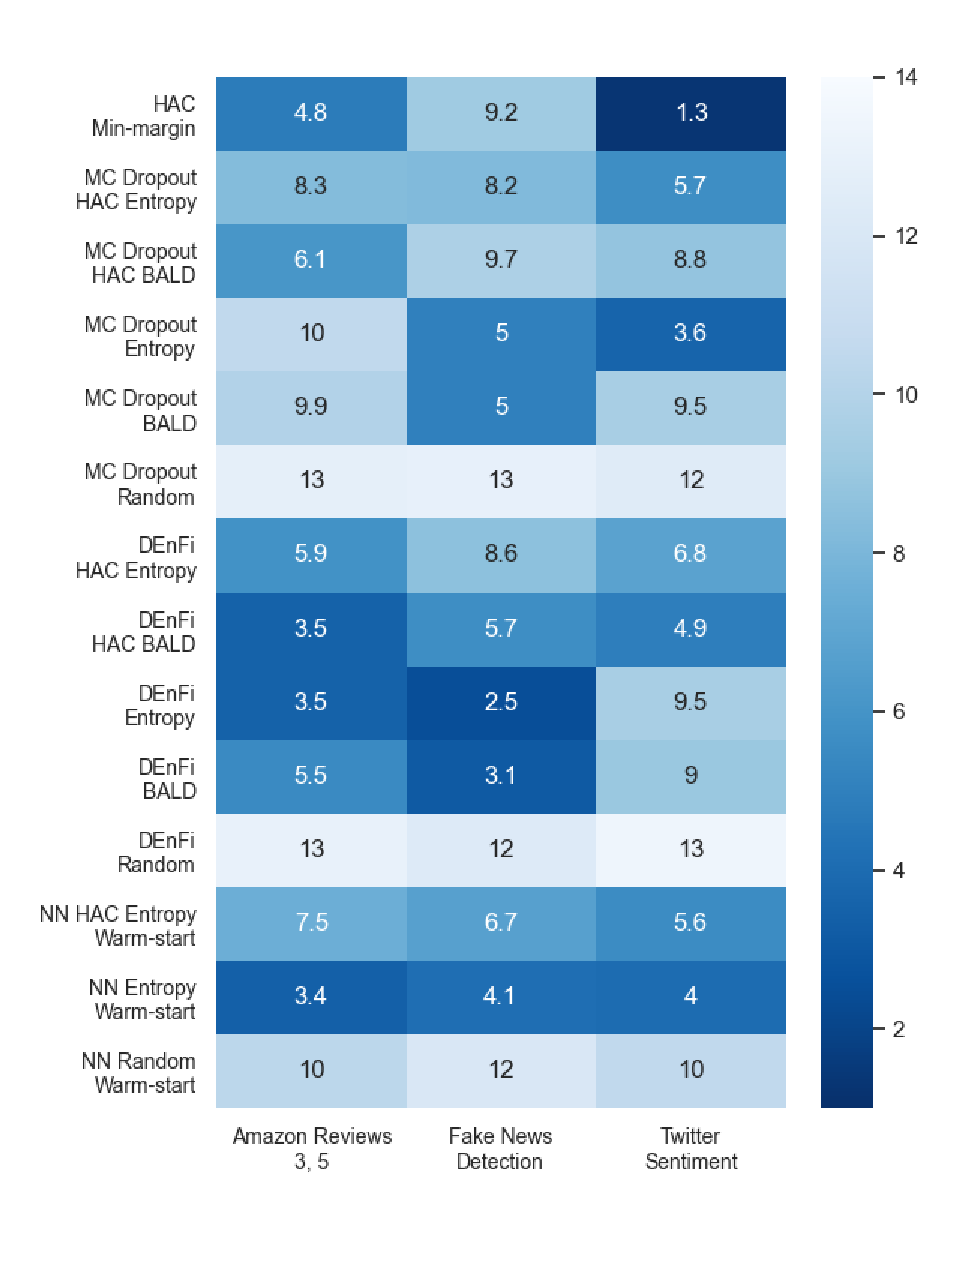
\includegraphics[scale=0.35]{images/Aggregated_mean_rank_given_datasets_w_denfi}
\par\end{centering}
\centering{}\caption{}
\end{figure}
\begin{figure*}
\begin{centering}
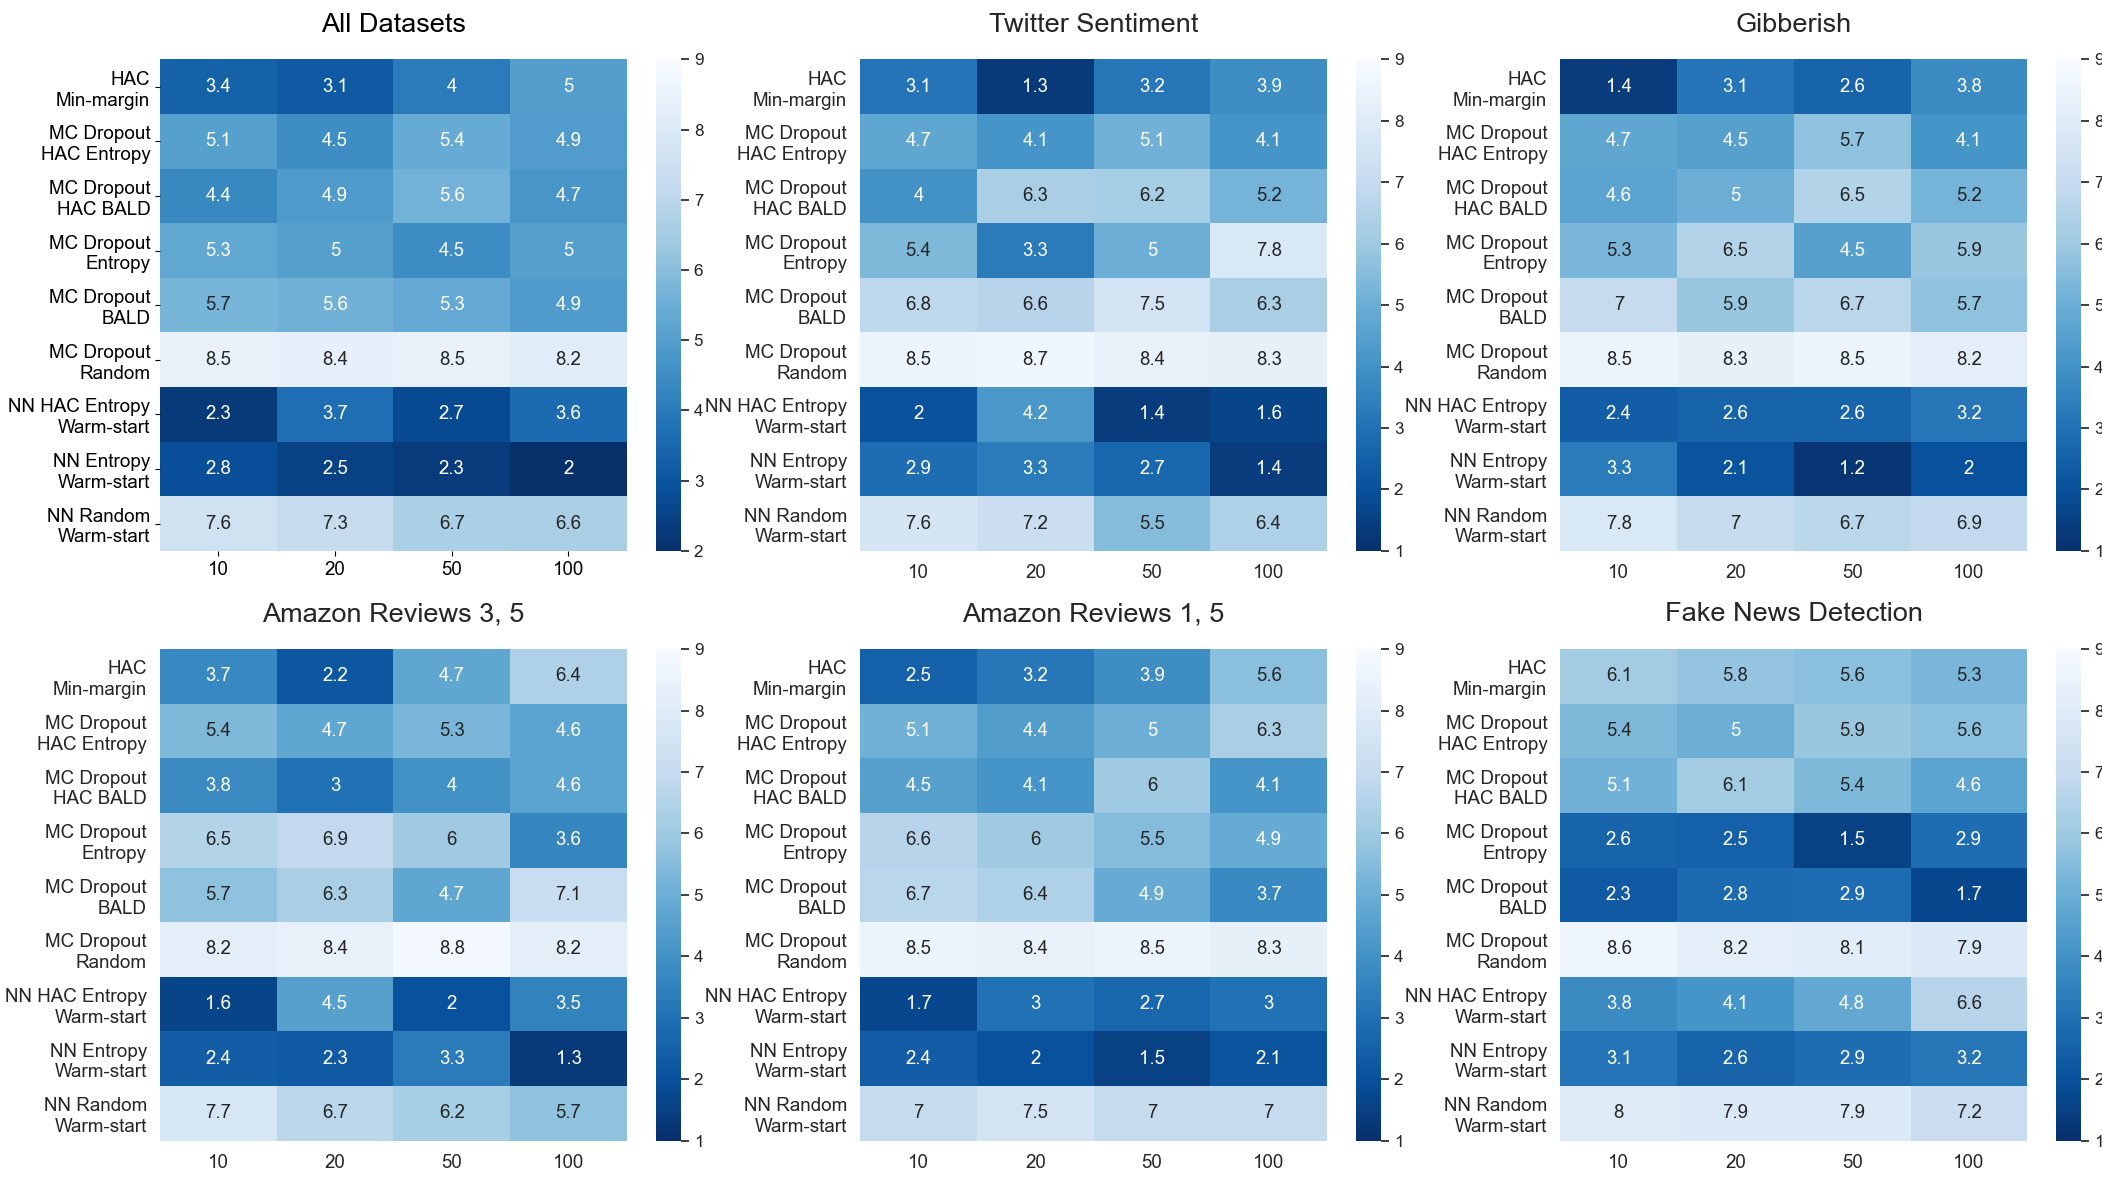
\includegraphics[scale=0.3]{images/Aggregated_mean_rank_given_datasets_subplots}
\par\end{centering}
\centering{}\caption{}
\end{figure*}

\begin{figure*}
\begin{centering}
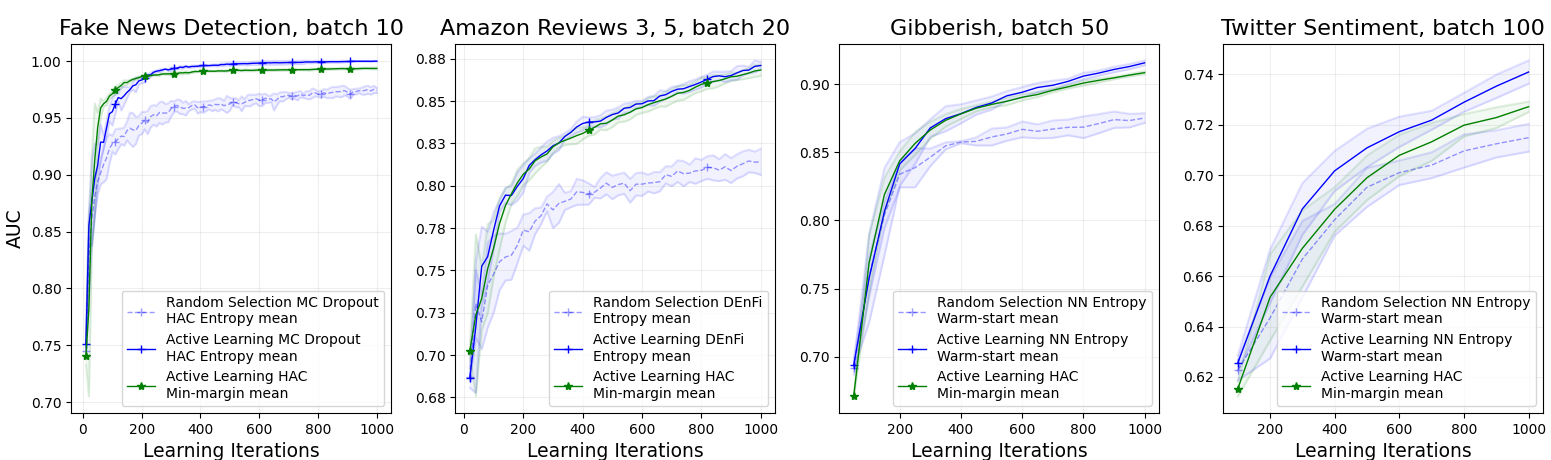
\includegraphics[scale=0.41]{images/batch_active_learning_plots}
\par\end{centering}
\centering{}\caption{}
\end{figure*}

\end{document}
